\subsection{Persistente Session Token Storage}\label{subsec:persistente-session-token-storage}
Collectiqo hatte Probleme mit der Nutzung von Session Variablen.
Diese wurden genutzt, um Variablen persistent zwischen Seitenwechseln und verschiedenen Funktionsaufrufen zu halten.
So wurde bspw. beim Login der Nutzername und die Nutzer-ID gesetzt, die dann bei verschiedenen HTTP Requests aufgerufen wurden.
Die vorherige Implementation war fehlerbehaftet und hat oftmals die Session Variablen nicht persistent gehalten.
Für dieses Semester wurde sich vorgenommen, die Implementierung zu verbessern.

Eine Lösung wurde in Form von einer Session Token Storage gefunden.
Im vorherigen Semester wurde bereits eine Mongo DB implementiert.
Aus verschiedenen Anleitung hat sich herauskristallisiert, dass eine Mongo DB geeignet ist für solch eine Session Toke Storage.
Es musste nur eine neue Collection hinzugefügt werden, auf welche dann in der Session Konfiguration in der app.js verwiesen wird:

\vspace{1em}
% \lstinputlisting[language=JavaScript, label={lst:session_storage}]{../../../src/app.js}
\vspace{1em}

Jegliche Session Variablen, die nun im Code gesetzt werden, werden in der Mongo DB gespeichert, in Verbindung mit dem Token.
Das Lesen und Speichern der Variablen wird automatisch von der Session Library übernommen, welches in der Datenbank dann wie folgt aussah:


\begin{figure}[h]
    \centering
    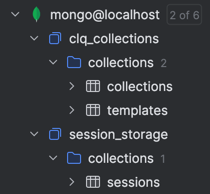
\includegraphics[width=0.5\textwidth]{session_storage_1}
    \caption{Struktur der Mongo DB}
    \label{fig:session:_storage_1}
\end{figure}


\begin{figure}[h]
    \centering
    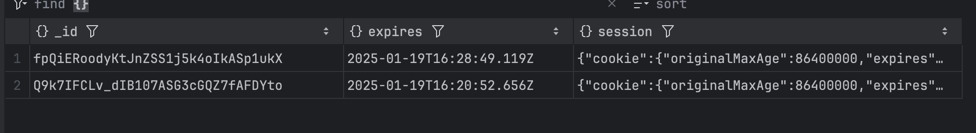
\includegraphics[width=0.5\textwidth]{session_storage_2}
    \caption{Tabellenansicht der Session Storage}
    \label{fig:session_storage_2}
\end{figure}